\section{System Evaluation}
\label{sec:evaluation}

\begin{figure}[!t]
\centering
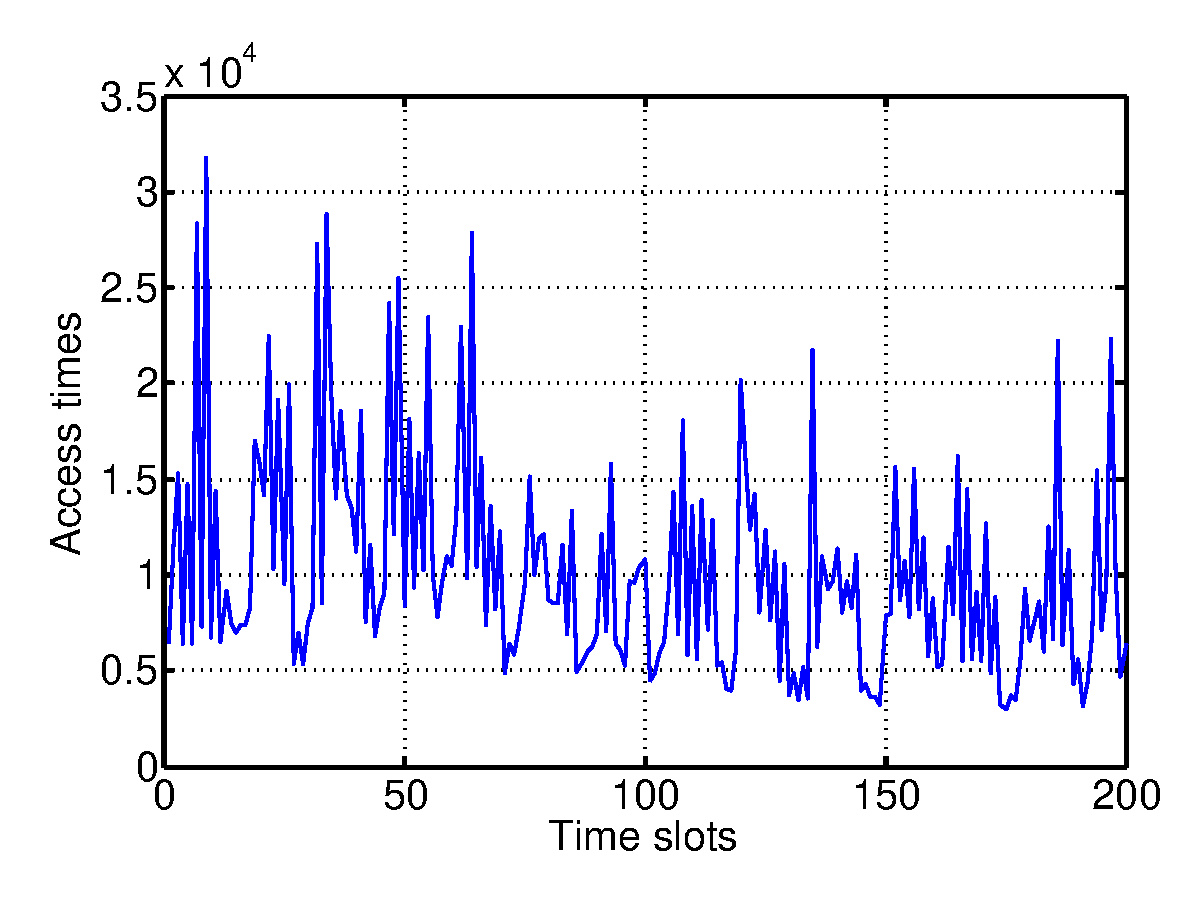
\includegraphics[width=2.0in]{./datafig1.pdf}
% where an .eps filename suffix will be assumed under latex,
% and a .pdf suffix will be assumed for pdflatex; or what has been declared
% via \DeclareGraphicsExtensions.
\caption{Illustration of Data Access Traces Type I}
\vspace{-0.1in}
\label{datafig1}
\end{figure}

\begin{figure}[!t]
\centering
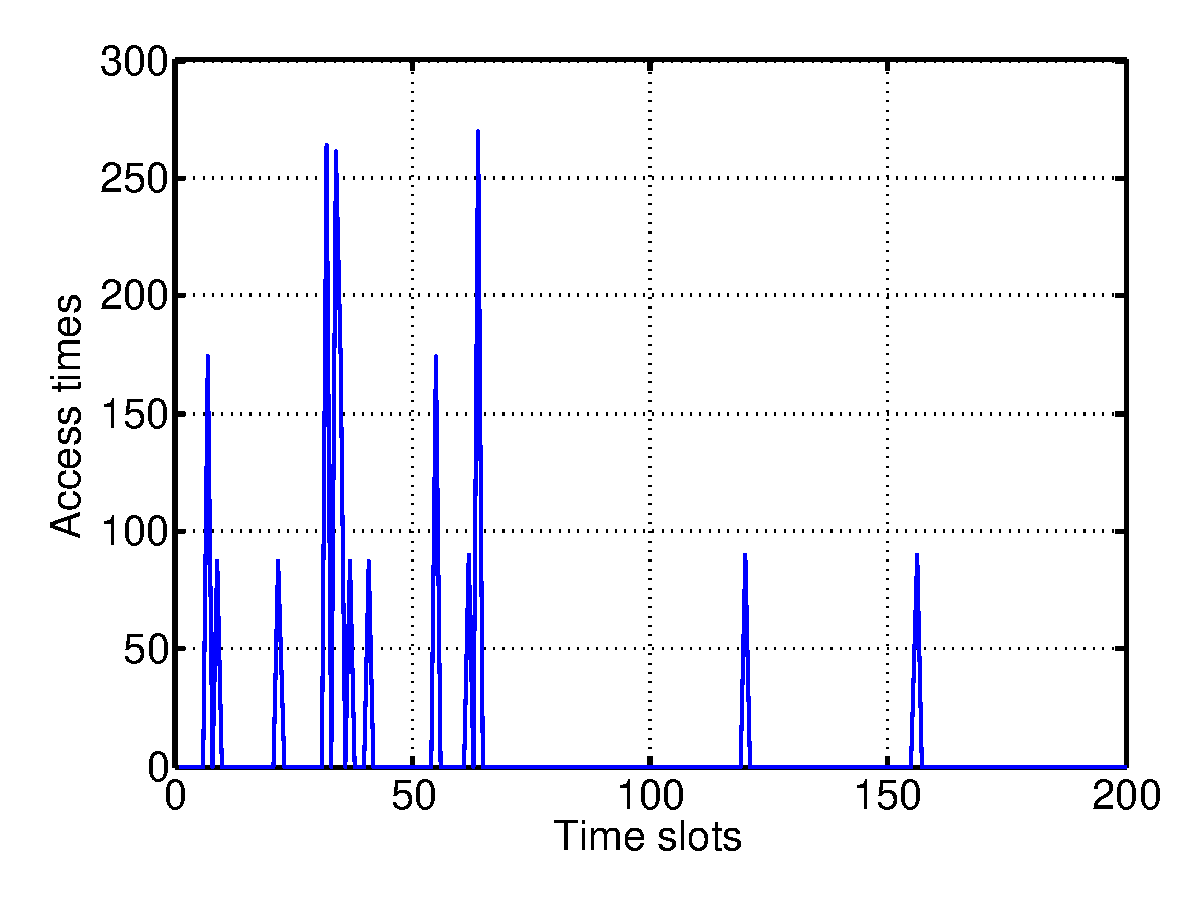
\includegraphics[width=2.0in]{./datafig2.pdf}
% where an .eps filename suffix will be assumed under latex,
% and a .pdf suffix will be assumed for pdflatex; or what has been declared
% via \DeclareGraphicsExtensions.
\caption{Illustration of Data Access Traces Type II}
\vspace{-0.25in}
\label{datafig2}
\end{figure}


In this section, we systematically present the evaluation of the proposed algorithm. We first present a study of the traces of data object accesses, based on which we evaluate the performance of our learning algorithm by replaying them. We use a long-term I/O traces, LASR traces~\cite{tracedata2}, which were collected at system-call level. We track the access frequency of different files during their lifetime. Specifically, we divide the time span into hundreds of time slots and each of which has same length. We then count how many times each file has been accessed during each time slot. In the LASR traces, we eliminate those files which have only been accessed less than 10 times during their lifetime (the access of these files almost has no impact on the performance of the storage system) and focus on the remaining ones (1,703 files) which are more frequently accessed. By analyzing the access of these frequently accessed files, we find out that these files can be roughly put into two categories according to their access patterns. The first category contains files that have constant access patterns. Files in this category have been frequently accessed during their whole lifetime, without too much difference between the maximum and minimum access periods. Fig.~\ref{datafig1} shows a typical file falls into this category. The learning algorithm, especially the Markov chain approach can achieve a higher level of accuracy for this kind of files. The second category is files with a bursty access pattern. Files in this category have only been accessed at very few time slots, but the access counts for those time slot can be very large. Fig.~\ref{datafig2} shows a typical file falling into this category. For files belong to second category, it is pretty hard for any learning algorithm including Markov chain approach to train a model to accurately predict their future access frequency.


To save the evaluation time, we did not use the entire LASR traces, instead, from the dataset we select traces of files that have been accessed more than 1,000 times (traces of 40 different files). For each trace we use the first half as the training data to train our Markov prediction model while use the other half as the testing data. As illustrated in Fig. \ref{prediction}, the bars represent the future access frequency of the 40 different files which are extracted from the testing dataset. Since we only have limited SSD storage space, our goal is to store the files that will be most frequently accessed in the future on SSD devices to improve the average data access throughput. For example, if we can only put 10 of 40 files on SSDs, as shown in Fig. \ref{prediction}, the light-colored bars illustrate the files predicted by our Markov model that are required to be placed on SSD devices. From the results we can observe that, 7 of 10 files that have the highest future access frequency have been chosen.

\begin{figure}[!t]
\centering
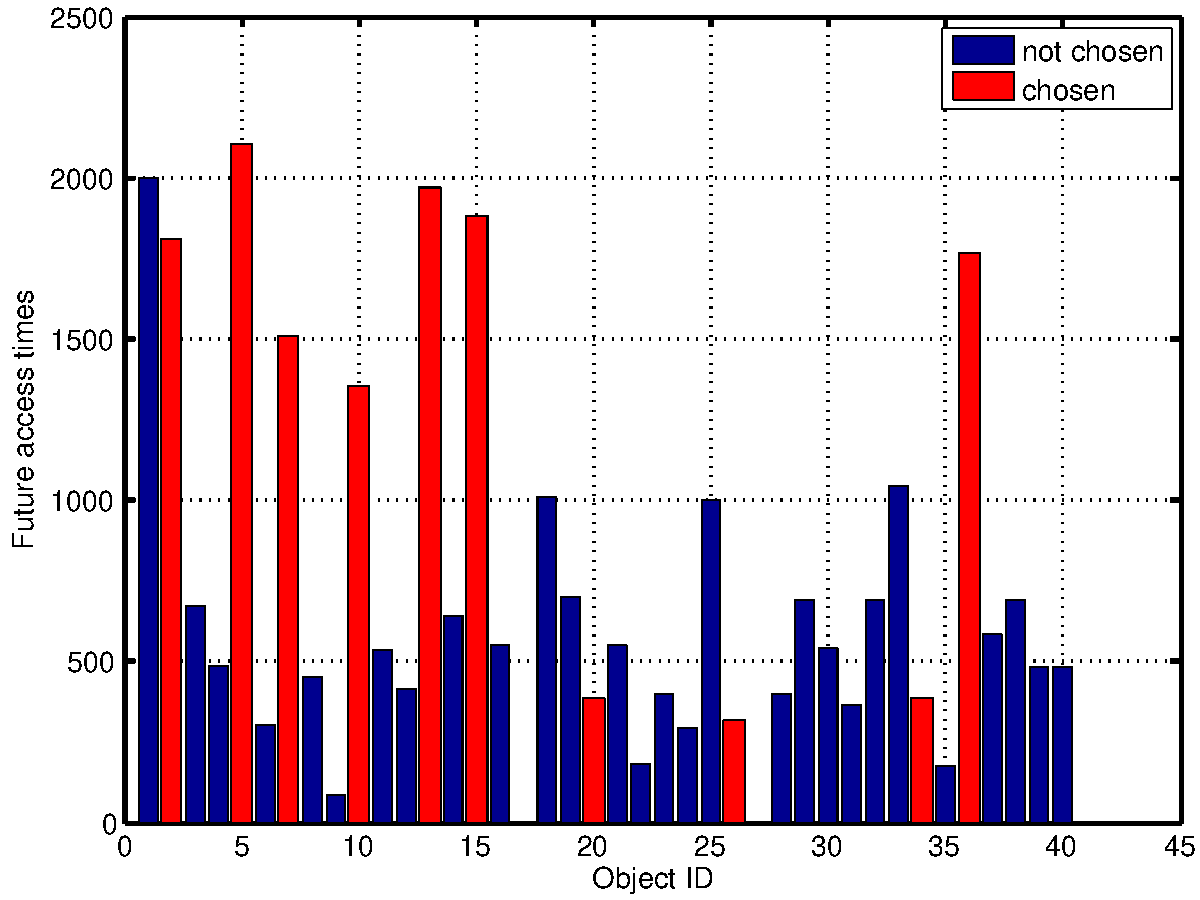
\includegraphics[width=2.4in]{./prediction.pdf}
% where an .eps filename suffix will be assumed under latex,
% and a .pdf suffix will be assumed for pdflatex; or what has been declared
% via \DeclareGraphicsExtensions.
\caption{Future Access Times of Data Objects}
\vspace{-0.1in}
\label{prediction}
\end{figure}

\begin{figure}[!t]
\centering
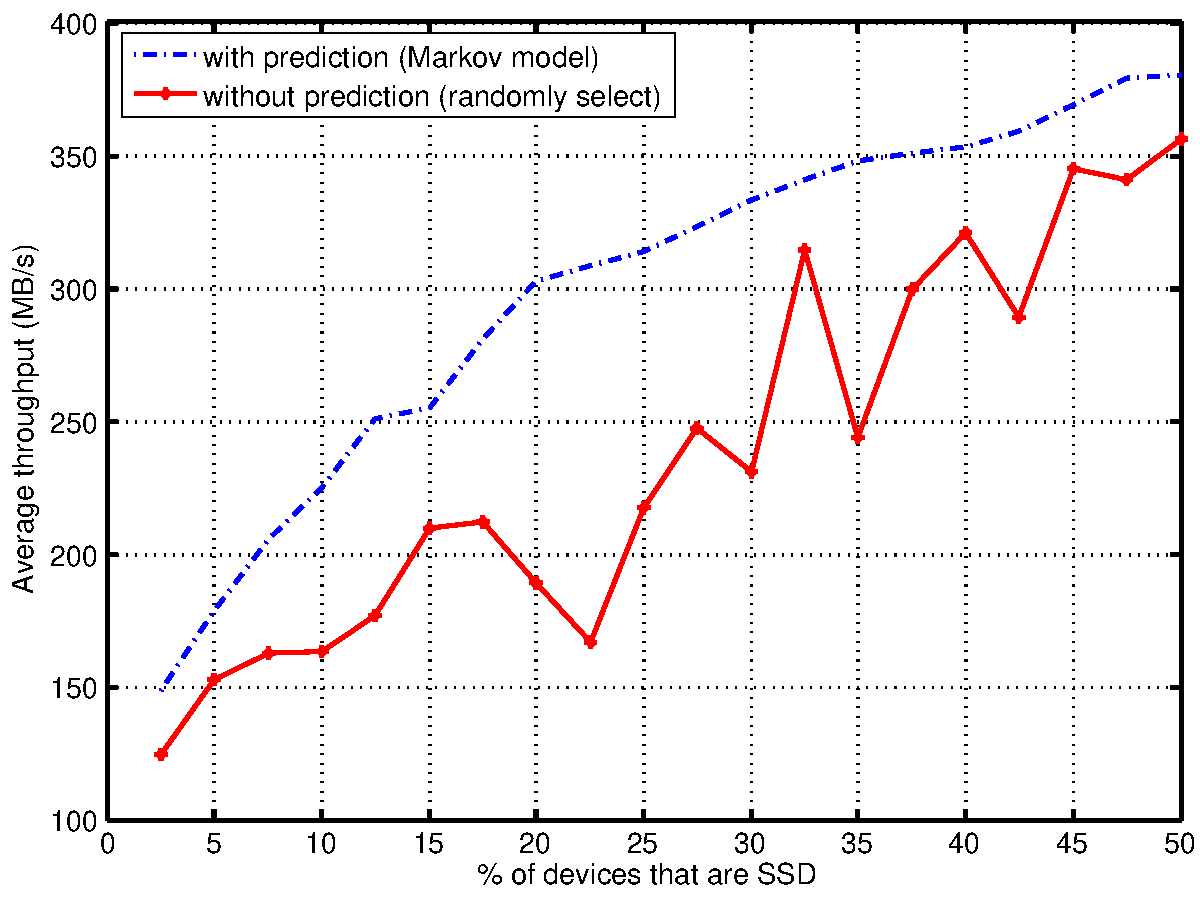
\includegraphics[width=2.4in]{./throughput.pdf}
% where an .eps filename suffix will be assumed under latex,
% and a .pdf suffix will be assumed for pdflatex; or what has been declared
% via \DeclareGraphicsExtensions.
\caption{Average Throughput v.s. Percentage of Objects Stored on SSDs}
\vspace{-0.25in}
\label{throughput}
\end{figure}

We next choose random selection approach as baseline and compare the average read throughput achieved by our Markov prediction model with that achieved by random object selection. Here the random object selection means that we randomly choose several data objects (files) and put them on SSD devices. The number of data objects that can be placed on SSD devices is also limited. For example, in the simulation, we vary the number of data objects that can be put on SSD devices from 2.5\% to 50\%. Besides, we set the read throughput of SSD devices as 550MB/s and that of HDD devices as 120 MB/s, consistent with typical datasheets provided by manufacturers of storage devices \cite{chen2009understanding}. As shown in Fig. \ref{throughput}, our object selection approach can achieve higher average read throughput than random selection, demonstrating the effectiveness of our proposed approaches.


